\sourcepageanchor{341}
\subsection{评价检验的方法}\label{sec:8.3}
实验者在决定接受或拒绝原假设 $H_0$ 时，可能犯错误. 通常通过犯错概率评价和比较假设检验. 本节讨论如何控制这些错误概率；有时甚至可以确定哪些检验具有尽可能小的错误概率.
\subsubsection{错误概率与功效函数}\label{sec:8.3.1}
检验 $H_0:\theta\in\Theta_0$ 对 $H_1:\theta\in\Theta_0^c$，可能犯两种错误中的一种. 传统上，这两种错误被赋予不易帮助记忆的名称：第一类错误（Type I Error）和第二类错误（Type II Error\mbox{）.} 若 $\theta\in\Theta_0$，检验却错误地决定拒绝 $H_0$，就犯了第一类错误. 反之，若 $\theta\in\Theta_0^c$，检验却决定接受 $H_0$，就犯了第二类错误. \autoref{tab:8.3.1}描述了这两种不同情形.

\begin{table}[htbp]\centering
\caption{假设检验中的两类错误}\label{tab:8.3.1}\index{SI0513@第一类错误}\index{SI0514@第二类错误}
\begin{tabular}{cc|cc}\toprule
&&\multicolumn{2}{c}{决策}\\
&&接受 $H_0$&拒绝 $H_0$\\\midrule
\multirow{2}{*}{真实状态}&$H_0$&正确决策&第一类错误\\
&$H_1$&第二类错误&正确决策\\\bottomrule
\end{tabular}
\end{table}

设 $R$ 表示某检验的拒绝域. 对 $\theta\in\Theta_0$，如果 $\boldsymbol x\in R$，检验就会犯错，故第一类错误的概率为 $P_\theta(\boldsymbol X\in R)$. 对 $\theta\in\Theta_0^c$，第二类错误的概率为 $P_\theta(\boldsymbol X\in R^c)$. 从 $R$ 转到 $R^c$ 略显混乱，但注意到 $P_\theta(\boldsymbol X\in R^c)=1-P_\theta(\boldsymbol X\in R)$，便知 $\theta$ 的函数 $P_\theta(\boldsymbol X\in R)$ 包含了有关拒绝域为 $R$ 的检验的全部信息. 有
$$P_\theta(\boldsymbol X\in R)=\begin{cases}\text{第一类错误的概率},&\theta\in\Theta_0,\\1-\text{第二类错误的概率},&\theta\in\Theta_0^c.\end{cases}$$
这一考虑引出如下定义.
\begin{definition}\label{def:8.3.1}\index{SI0501@功效}
拒绝域为 $R$ 的假设检验的功效函数（power function）是 $\theta$ 的函数 $\beta(\theta)=P_\theta(\boldsymbol X\in R)$.
\end{definition}
理想的功效函数对所有 $\theta\in\Theta_0$ 为零，对所有 $\theta\in\Theta_0^c$ 为一. 除平凡情形外，这一理想无法实现. 定性地说，好的检验应对大多数 $\theta\in\Theta_0^c$ 具有接近一的功效，对大多数 $\theta\in\Theta_0$ 具有接近零的功效.
\begin{example}[二项功效函数]\label{ex:8.3.2}\index{SI0502@二项}
设 $X\sim\operatorname{binomial}(5,\theta)$. 考虑检验 $H_0:\theta\le1/2$ 对 $H_1:\theta>1/2$. 先考虑仅在观察到全部“成功”时才拒绝 $H_0$ 的检验，其功效函数为
$$\beta_1(\theta)=P_\theta(\boldsymbol X\in R)=P_\theta(X=5)=\theta^5.$$
$\beta_1(\theta)$ 的图像见\autoref{fig:8.3.1}. 考察该功效函数，可能认为虽然第一类错误概率低到可以接受（对所有 $\theta\le1/2$，$\beta_1(\theta)\le(1/2)^5=.0312$），但对大多数 $\theta>1/2$，第二类错误概率太高（$\beta_1(\theta)$ 太小\mbox{）.} 只有当 $\theta>(1/2)^{1/5}=.87$ 时，第二类错误概率才小于 $1/2$. 为降低第二类错误概率，可以考虑在 $X=3,4,5$ 时拒绝 $H_0$ 的检验，其功效函数为
$$\begin{aligned}
\beta_2(\theta)&=P_\theta(X=3,4\text{ 或 }5)\\
&=\binom53\theta^3(1-\theta)^2+\binom54\theta^4(1-\theta)^1+\binom55\theta^5(1-\theta)^0.
\end{aligned}$$
\sourcepageanchor{342}

\begin{figure}[htbp]\centering
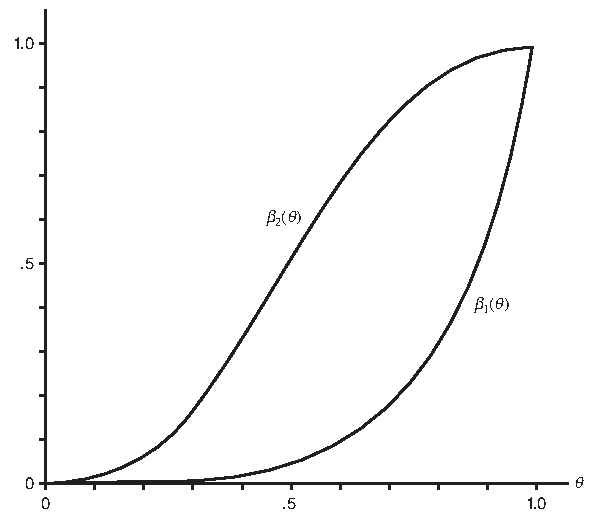
\includegraphics[width=.75\textwidth]{assets/chapter8/fig8-3-1.pdf}
\caption{\autoref{ex:8.3.2}的功效函数.}\label{fig:8.3.1}
\end{figure}

$\beta_2(\theta)$ 也画在\autoref{fig:8.3.1}中. 可见第二个检验确实减小了第二类错误概率，因为对 $\theta>1/2$，$\beta_2(\theta)$ 更大. 但第二个检验的第一类错误概率也更大，因为对 $\theta\le1/2$，$\beta_2(\theta)$ 也更大. 若要在两者之间选择，研究者必须决定哪一种错误结构——由 $\beta_1(\theta)$ 还是由 $\beta_2(\theta)$ 描述的结构——更可接受.
\end{example}
\begin{example}[正态功效函数]\label{ex:8.3.3}\index{SI0504@正态}
设 $X_1,\ldots,X_n$ 是来自 $\mathrm n(\theta,\sigma^2)$ 总体的随机样本，$\sigma^2$ 已知. 检验 $H_0:\theta\le\theta_0$ 对 $H_1:\theta>\theta_0$ 的一种似然比检验，是当 $(\bar X-\theta_0)/(\sigma/\sqrt n)>c$ 时拒绝 $H_0$（\autoref{exercise:8.37}\mbox{）.} 常数 $c$ 可以是任意正数. 其功效函数为
$$\begin{aligned}
\beta(\theta)&=P_\theta\left(\frac{\bar X-\theta_0}{\sigma/\sqrt n}>c\right)\\
&=P_\theta\left(\frac{\bar X-\theta}{\sigma/\sqrt n}>c+\frac{\theta_0-\theta}{\sigma/\sqrt n}\right)\\
&=P\left(Z>c+\frac{\theta_0-\theta}{\sigma/\sqrt n}\right),
\end{aligned}$$
其中 $Z$ 为标准正态随机变量，因为 $(\bar X-\theta)/(\sigma/\sqrt n)\sim\mathrm n(0,1)$. 容易看出，当 $\theta$ 从 $-\infty$ 增至 $\infty$ 时，这一正态概率从零增至一. 因此 $\beta(\theta)$ 是 $\theta$ 的增函数，并且
$$\lim_{\theta\to-\infty}\beta(\theta)=0,\qquad\lim_{\theta\to\infty}\beta(\theta)=1,\qquad
\beta(\theta_0)=\alpha\ \text{若 }P(Z>c)=\alpha.$$
\autoref{fig:8.3.2}给出了 $c=1.28$ 时的 $\beta(\theta)$ 图像.
\end{example}
通常，检验的功效函数依赖样本量 $n$. 若 $n$ 可由实验者选择，考虑功效函数就可能帮助确定实验中适当的样本量.
\sourcepageanchor{343}

\begin{figure}[htbp]\centering
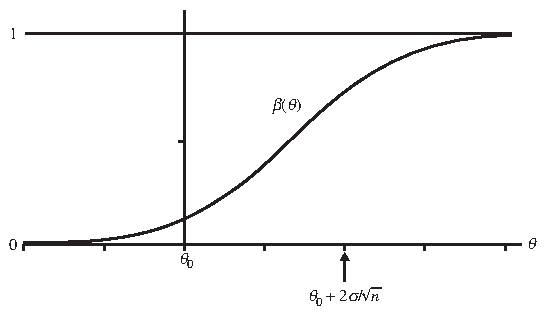
\includegraphics[width=.78\textwidth]{assets/chapter8/fig8-3-2.pdf}
\caption{\autoref{ex:8.3.3}的功效函数.}\label{fig:8.3.2}
\end{figure}

\begin{example}[续\autoref{ex:8.3.3}]\label{ex:8.3.4}\index{SI0510@正态}\index{SI0513@第一类错误}\index{SI0514@第二类错误}\index{SI0947@假设检验：正态}
假设实验者希望最大第一类错误概率为 $.1$；此外，希望在 $\theta\ge\theta_0+\sigma$ 时，最大第二类错误概率为 $.2$. 现在说明如何选择 $c$ 和 $n$ 达到这些目标，采用的检验是在 $(\bar X-\theta_0)/(\sigma/\sqrt n)>c$ 时拒绝 $H_0:\theta\le\theta_0$. 如上所述，这种检验的功效函数为
$$\beta(\theta)=P\left(Z>c+\frac{\theta_0-\theta}{\sigma/\sqrt n}\right).$$
由于 $\beta(\theta)$ 随 $\theta$ 递增，只要
$$\beta(\theta_0)=.1\quad\text{且}\quad\beta(\theta_0+\sigma)=.8,$$
就满足要求.

选择 $c=1.28$，无论 $n$ 为何，都有 $\beta(\theta_0)=P(Z>1.28)=.1$. 现在要选取 $n$，使 $\beta(\theta_0+\sigma)=P(Z>1.28-\sqrt n)=.8$. 因 $P(Z>-.84)=.8$，令 $1.28-\sqrt n=-.84$，解得 $n=4.49$. 当然，$n$ 必须是整数，所以取 $c=1.28$、$n=5$，即可按实验者的规定控制错误概率.\footnote{译注：这里的正态分位数和概率均经过舍入，原文用等号表示近似值. 实际上 $P(Z>1.28)\approx.10027$，略大于 $.1$；若要求严格不超过 $.1$，应取 $c=z_{.1}\approx1.28155$，此时取 $n=5$ 仍满足第二类错误的要求.}
\end{example}
样本量固定时，通常不可能把两类错误概率都任意缩小. 寻找好的检验时，通常先把考虑范围限制为能将第一类错误概率控制在指定水平的检验，再在这一类中寻找第二类错误概率尽可能小的检验. 讨论第一类错误概率的控制时，下列两个术语很有用.
\begin{definition}\label{def:8.3.5}\index{SI0511@检验大小}
对 $0\le\alpha\le1$，若功效函数为 $\beta(\theta)$ 的检验满足 $\sup_{\theta\in\Theta_0}\beta(\theta)=\alpha$，则称其为大小为 $\alpha$ 的检验（size $\alpha$ test\mbox{）.}
\end{definition}
\begin{definition}\label{def:8.3.6}\index{SI0498@检验水平}
对 $0\le\alpha\le1$，若功效函数为 $\beta(\theta)$ 的检验满足 $\sup_{\theta\in\Theta_0}\beta(\theta)\le\alpha$，则称其为水平为 $\alpha$ 的检验（level $\alpha$ test\mbox{）.}
\end{definition}
有些作者不像我们这样区分大小（size）与水平（level），有时两词互换使用. 但按本书的定义，水平为 $\alpha$ 的检验集合包含大小为 $\alpha$ 的检验集合. 而且，在复杂模型和复杂检验问题中，这一区别很重要，因为计算上往往无法构造大小恰为 $\alpha$ 的检验. 此时实验者必须满足于水平为 $\alpha$ 的检验，意识到可能需要某些折中.
\sourcepageanchor{344}
后面会看到一些例子，特别是在并交检验和交并检验中.

实验者通常指定所用检验的水平，典型选择为 $\alpha=.01,.05,.10$. 要注意，固定检验水平只控制第一类错误概率，并不控制第二类错误. 采用这种方法时，应恰当设置原假设和备择假设，使控制第一类错误概率成为最重要的事情. 例如，某实验者期待实验支持一个特定假设，但除非数据确实给出令人信服的支持，否则不愿作出断言. 可以把检验设置成：备择假设正是她期待数据支持、希望证明的假设. （在这一语境下，备择假设有时称为研究假设（research hypothesis\mbox{）.}\index{SI0479@研究}\semanticindexanchor{479:344}）通过采用 $\alpha$ 较小的水平 $\alpha$ 检验，她就能防范在研究假设为假时声称数据支持它.

\autoref{sec:8.2}的方法通常给出检验统计量和拒绝域的一般形式，却通常不会确定某一个具体检验. 例如，似然比检验（\autoref{def:8.2.1}）在 $\lambda(\boldsymbol X)\le c$ 时拒绝 $H_0$，但 $c$ 未指定，所以定义的是整类似然比检验，每个 $c$ 值对应一个. 现在将范围限制为大小 $\alpha$ 的检验，就可能从中选出一个.
\begin{example}[似然比检验的大小]\label{ex:8.3.7}\index{SI0634@指数}\index{SI0638@正态}
一般地，选择 $c$ 使 $\sup_{\theta\in\Theta_0}P_\theta(\lambda(\boldsymbol X)\le c)=\alpha$，便构造出大小为 $\alpha$ 的似然比检验. 如何确定 $c$，依具体问题而定. 例如，在\autoref{ex:8.2.2}中，$\Theta_0$ 只含单点 $\theta=\theta_0$，且在此点 $\sqrt n(\bar X-\theta_0)\sim\mathrm n(0,1)$. 因而，检验
$$\text{若 }|\bar X-\theta_0|\ge z_{\alpha/2}/\sqrt n,\quad\text{则拒绝 }H_0,$$
就是大小为 $\alpha$ 的似然比检验；其中 $z_{\alpha/2}$ 满足 $P(Z\ge z_{\alpha/2})=\alpha/2$，$Z\sim\mathrm n(0,1)$. 具体而言，这相当于取 $c=\exp(-z_{\alpha/2}^2/2)$，但这一点并不重要.

对\autoref{ex:8.2.3}的问题，原假设 $H_0:\theta\le\theta_0$ 包含不止一个点，因此寻找大小为 $\alpha$ 的似然比检验更加复杂. 检验在 $X_{(1)}\ge c$ 时拒绝 $H_0$，其中 $c$ 应使检验大小为 $\alpha$. 但若 $c=(-\log\alpha)/n+\theta_0$，则
$$P_{\theta_0}(X_{(1)}\ge c)=e^{-n(c-\theta_0)}=\alpha.$$
由于 $\theta$ 是 $X_{(1)}$ 的位置参数，
$$P_\theta(X_{(1)}\ge c)\le P_{\theta_0}(X_{(1)}\ge c),\qquad\text{对任意 }\theta\le\theta_0.$$
因此，
$$\sup_{\theta\in\Theta_0}\beta(\theta)=\sup_{\theta\le\theta_0}P_\theta(X_{(1)}\ge c)
=P_{\theta_0}(X_{(1)}\ge c)=\alpha,$$
这个 $c$ 就给出了大小为 $\alpha$ 的似然比检验.
\end{example}
\emph{记号说明：}上例用 $z_{\alpha/2}$ 表示标准正态密度曲线下右侧概率为 $\alpha/2$ 的点. 我们将普遍使用这种记法，不仅用于正态分布，也用于其他分布（为清楚起见，会按需给出定义\mbox{）.} 例如，$z_\alpha$ 满足 $P(Z>z_\alpha)=\alpha$，其中 $Z\sim\mathrm n(0,1)$；$t_{n-1,\alpha/2}$ 满足 $P(T_{n-1}>t_{n-1,\alpha/2})=\alpha/2$，其中 $T_{n-1}\sim t_{n-1}$；$\chi^2_{p,1-\alpha}$ 满足 $P(\chi_p^2>\chi^2_{p,1-\alpha})=1-\alpha$，其中 $\chi_p^2$ 是自由度为 $p$ 的卡方随机变量. $z_{\alpha/2},z_\alpha,t_{n-1,\alpha/2},\chi^2_{p,1-\alpha}$ 等点称为临界点（cutoff points\mbox{）.}\index{SI0243@临界点}\semanticindexanchor{243:344}
\begin{example}[并交检验的大小]\label{ex:8.3.8}\index{SI0525@正态}\index{SI1028@并交}
在\autoref{ex:8.2.8}中，寻找大小为 $\alpha$ 的并交检验，就是寻找常数 $t_L,t_U$，使
$$\sup_{\theta\in\Theta_0}P_\theta\left(\frac{\bar X-\mu_0}{\sqrt{S^2/n}}\ge t_L\quad\text{或}\quad\frac{\bar X-\mu_0}{\sqrt{S^2/n}}\le t_U\right)=\alpha.$$
\sourcepageanchor{345}
但对任意 $(\mu,\sigma^2)=\theta\in\Theta_0$，都有 $\mu=\mu_0$，因此 $(\bar X-\mu_0)/\sqrt{S^2/n}$ 服从自由度为 $n-1$ 的 Student $t$ 分布. 所以，只要取 $t_U=t_{n-1,1-\alpha_1}$、$t_L=t_{n-1,\alpha_2}$，其中 $\alpha_1+\alpha_2=\alpha$，就得到对所有 $\theta\in\Theta_0$ 第一类错误概率均恰为 $\alpha$ 的检验. 通常取 $t_L=-t_U=t_{n-1,\alpha/2}$.
\end{example}
除了 $\alpha$ 水平，还可能关心检验的其他特征. 例如，希望在 $\theta\in\Theta_0^c$ 时，比在 $\theta\in\Theta_0$ 时更可能拒绝 $H_0$. \autoref{fig:8.3.1}和\autoref{fig:8.3.2}的全部功效函数都有此性质，得到的检验称为无偏检验.
\begin{definition}\label{def:8.3.9}\index{SI0520@无偏}
若对每个 $\theta'\in\Theta_0^c$ 和 $\theta''\in\Theta_0$，都有 $\beta(\theta')\ge\beta(\theta'')$，则功效函数为 $\beta(\theta)$ 的检验称为无偏的（unbiased\mbox{）.}
\end{definition}
\begin{example}[\autoref{ex:8.3.3}的结论]\label{ex:8.3.10}
检验 $H_0:\theta\le\theta_0$ 对 $H_1:\theta>\theta_0$ 的似然比检验具有功效函数
$$\beta(\theta)=P\left(Z>c+\frac{\theta_0-\theta}{\sigma/\sqrt n}\right),$$
其中 $Z\sim\mathrm n(0,1)$. 由于对固定 $\theta_0$，$\beta(\theta)$ 是 $\theta$ 的增函数，故
$$\beta(\theta)>\beta(\theta_0)=\max_{t\le\theta_0}\beta(t),\qquad\text{对所有 }\theta>\theta_0,$$
所以该检验无偏.
\end{example}
多数问题有许多无偏检验（见\autoref{exercise:8.45}\mbox{）.} 同样，大小为 $\alpha$ 的检验、似然比检验等也往往有许多个. 有时施加的限制已足以把考虑范围缩减为一个检验. \autoref{ex:8.3.7}中的两个问题，都只有一个大小为 $\alpha$ 的似然比检验. 在其他情形下，仍有许多检验可选；我们只讨论了在 $T$ 较大时拒绝 $H_0$ 的那一个. 接下来将讨论从一类检验中作选择的其他准则，它们都与检验的功效函数有关.

\subsubsection{最强检验}\label{sec:8.3.2}
前几节描述了各种假设检验类. 其中一些控制第一类错误概率，例如水平为 $\alpha$ 的检验对所有 $\theta\in\Theta_0$ 都使第一类错误概率不超过 $\alpha$. 这类中的好检验还应具有较小的第二类错误概率，即在 $\theta\in\Theta_0^c$ 时功效函数较大. 若一个检验的第二类错误概率比类中所有其他检验都小，它当然有力地竞争着类中最佳检验的地位. 下列定义将这一想法形式化.
\begin{definition}\label{def:8.3.11}\index{SI0515@一致最强}
设 $\mathscr C$ 是检验 $H_0:\theta\in\Theta_0$ 对 $H_1:\theta\in\Theta_0^c$ 的一个检验类. 类 $\mathscr C$ 中功效函数为 $\beta(\theta)$ 的检验，若对每个 $\theta\in\Theta_0^c$，以及类 $\mathscr C$ 中每个检验的功效函数 $\beta'(\theta)$，都有 $\beta(\theta)\ge\beta'(\theta)$，就称为类 $\mathscr C$ 中的一致最强检验（uniformly most powerful，UMP\mbox{）.}
\end{definition}
本节中，$\mathscr C$ 取全部水平 $\alpha$ 检验构成的类，\autoref{def:8.3.11}中的检验于是称为水平 $\alpha$ 的一致最强检验. 要使这种检验有意义，对 $\mathscr C$ 的限制必须包含对第一类错误概率的某种限制. 完全不控制第一类错误概率而使第二类错误概率最小，并没有多大意义. （例如，以概率 $1$ 拒绝 $H_0$ 的检验永远不会犯第二类错误，见\autoref{exercise:8.16}.）

\autoref{def:8.3.11}要求很强，许多实际问题中不存在一致最强检验. 但在存在时，它完全可以被视为类中最佳检验. 因此，我们希望能识别出存在的一致最强检验. 下面著名的定理明确指出：当原假设和备择假设各自只包含样本的一种概率分布，即二者均为简单假设时\index{SI0480@简单}\semanticindexanchor{480:345}，哪些检验是水平 $\alpha$ 的一致最强检验.
\sourcepageanchor{346}
\begin{theorem}[Neyman–Pearson 引理]\label{thm:8.3.12}\index{SI0722@Neyman–Pearson引理}
考虑检验 $H_0:\theta=\theta_0$ 对 $H_1:\theta=\theta_1$，$\theta_i$ 对应的密度或质量函数为 $f(\boldsymbol x\mid\theta_i)$，$i=0,1$. 使用拒绝域为 $R$ 的检验，满足对某个 $k\ge0$，
\begin{equation}\label{eq:8.3.1}
\begin{aligned}
\boldsymbol x\in R&\quad\text{若 }f(\boldsymbol x\mid\theta_1)>kf(\boldsymbol x\mid\theta_0),\\
\text{且}\qquad\boldsymbol x\in R^c&\quad\text{若 }f(\boldsymbol x\mid\theta_1)<kf(\boldsymbol x\mid\theta_0),
\end{aligned}
\end{equation}
以及
\begin{equation}\label{eq:8.3.2}\alpha=P_{\theta_0}(\boldsymbol X\in R).\end{equation}
则
\begin{enumerate}
\item\phantomsection\label{itm:thm:8.3.12:a}（充分性）任何满足\eqref{eq:8.3.1}和\eqref{eq:8.3.2}的检验，都是水平 $\alpha$ 的一致最强检验.
\item\phantomsection\label{itm:thm:8.3.12:b}（必要性）若存在满足\eqref{eq:8.3.1}、\eqref{eq:8.3.2}且 $k>0$ 的检验，则每个水平 $\alpha$ 的一致最强检验大小都为 $\alpha$（满足\eqref{eq:8.3.2}）；并且每个水平 $\alpha$ 的一致最强检验都满足\eqref{eq:8.3.1}，至多在某个满足 $P_{\theta_0}(\boldsymbol X\in A)=P_{\theta_1}(\boldsymbol X\in A)=0$ 的集合 $A$ 上例外.
\end{enumerate}
\end{theorem}
\begin{proof}
我们证明 $f(\boldsymbol x\mid\theta_0)$ 和 $f(\boldsymbol x\mid\theta_1)$ 是连续随机变量密度的情形. 离散情形的证明只需把积分换成求和（见\autoref{exercise:8.21}\mbox{）.}

首先注意，任何满足\eqref{eq:8.3.2}的检验，大小都为 $\alpha$，从而水平也为 $\alpha$，因为 $\Theta_0$ 只有一个点，故 $\sup_{\theta\in\Theta_0}P_\theta(\boldsymbol X\in R)=P_{\theta_0}(\boldsymbol X\in R)=\alpha$.

为简化记号，定义检验函数（test function）\index{SI1032@检验函数}\semanticindexanchor{1032:346}：它是样本空间上的函数，在 $\boldsymbol x\in R$ 时为 $1$，在 $\boldsymbol x\in R^c$ 时为 $0$，即拒绝域的示性函数. 设 $\phi(\boldsymbol x)$ 是满足\eqref{eq:8.3.1}与\eqref{eq:8.3.2}的检验的检验函数，$\phi'(\boldsymbol x)$ 是任一其他水平 $\alpha$ 检验的检验函数，$\beta(\theta)$ 与 $\beta'(\theta)$ 分别为二者的功效函数. 因为 $0\le\phi'(\boldsymbol x)\le1$，\eqref{eq:8.3.1}蕴含对每个 $\boldsymbol x$，
$$[\phi(\boldsymbol x)-\phi'(\boldsymbol x)][f(\boldsymbol x\mid\theta_1)-kf(\boldsymbol x\mid\theta_0)]\ge0$$
（因为当 $f(\boldsymbol x\mid\theta_1)>kf(\boldsymbol x\mid\theta_0)$ 时 $\phi=1$，当反向严格不等式成立时 $\phi=0$\mbox{）.} 因此，
\begin{equation}\label{eq:8.3.3}
\begin{aligned}
0&\le\int[\phi(\boldsymbol x)-\phi'(\boldsymbol x)][f(\boldsymbol x\mid\theta_1)-kf(\boldsymbol x\mid\theta_0)]\,d\boldsymbol x\\
&=\beta(\theta_1)-\beta'(\theta_1)-k[\beta(\theta_0)-\beta'(\theta_0)].
\end{aligned}
\end{equation}
为证明\hyperref[itm:thm:8.3.12:a]{(a)}，注意 $\phi'$ 的水平为 $\alpha$ 而 $\phi$ 的大小为 $\alpha$，故 $\beta(\theta_0)-\beta'(\theta_0)=\alpha-\beta'(\theta_0)\ge0$. 因而\eqref{eq:8.3.3}与 $k\ge0$ 蕴含
$$0\le\beta(\theta_1)-\beta'(\theta_1)-k[\beta(\theta_0)-\beta'(\theta_0)]\le\beta(\theta_1)-\beta'(\theta_1),$$
表明 $\beta(\theta_1)\ge\beta'(\theta_1)$，即 $\phi$ 的功效不低于 $\phi'$. 因 $\phi'$ 是任意水平 $\alpha$ 的检验，$\theta_1$ 又是 $\Theta_0^c$ 中的唯一点，所以 $\phi$ 是水平 $\alpha$ 的一致最强检验.

为证明\hyperref[itm:thm:8.3.12:b]{(b)}，现令 $\phi'$ 为任一水平 $\alpha$ 的一致最强检验的检验函数. 由\hyperref[itm:thm:8.3.12:a]{(a)}，满足\eqref{eq:8.3.1}和\eqref{eq:8.3.2}的 $\phi$ 也是水平 $\alpha$ 的一致最强检验，故 $\beta(\theta_1)=\beta'(\theta_1)$. 这一事实、\eqref{eq:8.3.3}以及 $k>0$ 蕴含
$$\alpha-\beta'(\theta_0)=\beta(\theta_0)-\beta'(\theta_0)\le0.$$
由于 $\phi'$ 的水平为 $\alpha$，又有 $\beta'(\theta_0)\le\alpha$. 所以 $\beta'(\theta_0)=\alpha$，即 $\phi'$ 的大小为 $\alpha$，且\eqref{eq:8.3.3}此时取等号. 然而，非负被积函数 $[\phi(\boldsymbol x)-\phi'(\boldsymbol x)][f(\boldsymbol x\mid\theta_1)-kf(\boldsymbol x\mid\theta_0)]$ 的积分只有在 $\phi'$ 满足\eqref{eq:8.3.1}时才为零，至多在某个满足 $\int_Af(\boldsymbol x\mid\theta_i)\,d\boldsymbol x=0$ 的集合 $A$ 上例外. 这就证明了\hyperref[itm:thm:8.3.12:b]{(b)}的最后一个断言.
\end{proof}
\sourcepageanchor{347}
下面的推论把 Neyman–Pearson 引理与充分性联系起来.
\begin{corollary}\label{cor:8.3.13}\index{SI0512@充分性}
考虑\autoref{thm:8.3.12}中的假设检验问题. 设 $T(\boldsymbol X)$ 是 $\theta$ 的充分统计量，$g(t\mid\theta_i)$ 是 $T$ 在 $\theta_i$ 下的密度或质量函数，$i=0,1$. 则基于 $T$、拒绝域为 $S$（$T$ 的样本空间的一个子集）的任一检验，只要对某个 $k\ge0$ 满足
\begin{equation}\label{eq:8.3.4}
\begin{aligned}t\in S&\quad\text{若 }g(t\mid\theta_1)>kg(t\mid\theta_0),\\
\text{且}\qquad t\in S^c&\quad\text{若 }g(t\mid\theta_1)<kg(t\mid\theta_0),\end{aligned}
\end{equation}
就是水平 $\alpha$ 的一致最强检验，其中
\begin{equation}\label{eq:8.3.5}\alpha=P_{\theta_0}(T\in S).\end{equation}
\end{corollary}
\begin{proof}
用原样本 $\boldsymbol X$ 表示，基于 $T$ 的检验的拒绝域为 $R=\{\boldsymbol x:T(\boldsymbol x)\in S\}$. 由因子分解定理，可将 $\boldsymbol X$ 的密度或质量函数写为 $f(\boldsymbol x\mid\theta_i)=g(T(\boldsymbol x)\mid\theta_i)h(\boldsymbol x)$，$i=0,1$，其中 $h(\boldsymbol x)$ 非负. 将\eqref{eq:8.3.4}的不等式乘以这一非负函数，就看到 $R$ 满足
$$\boldsymbol x\in R\quad\text{若 }f(\boldsymbol x\mid\theta_1)=g(T(\boldsymbol x)\mid\theta_1)h(\boldsymbol x)>kg(T(\boldsymbol x)\mid\theta_0)h(\boldsymbol x)=kf(\boldsymbol x\mid\theta_0),$$
以及
$$\boldsymbol x\in R^c\quad\text{若 }f(\boldsymbol x\mid\theta_1)=g(T(\boldsymbol x)\mid\theta_1)h(\boldsymbol x)<kg(T(\boldsymbol x)\mid\theta_0)h(\boldsymbol x)=kf(\boldsymbol x\mid\theta_0).$$
另外，由\eqref{eq:8.3.5}，
$$P_{\theta_0}(\boldsymbol X\in R)=P_{\theta_0}(T(\boldsymbol X)\in S)=\alpha.$$
所以，由 Neyman–Pearson 引理的充分性部分，基于 $T$ 的检验是水平 $\alpha$ 的一致最强检验.
\end{proof}
推导满足\eqref{eq:8.3.1}或\eqref{eq:8.3.4}、从而为水平 $\alpha$ 的一致最强检验时，通常把不等式改写为 $f(\boldsymbol x\mid\theta_1)/f(\boldsymbol x\mid\theta_0)>k$ 更方便（须留意除数为零的情形\mbox{）.} 以下例子采用这种方法.
\begin{example}[二项总体的一致最强检验]\label{ex:8.3.14}\index{SI0516@二项}
设 $X\sim\operatorname{binomial}(2,\theta)$. 要检验 $H_0:\theta=1/2$ 对 $H_1:\theta=3/4$. 计算概率质量函数之比，得到
$$\frac{f(0\mid\theta=3/4)}{f(0\mid\theta=1/2)}=\frac14,\qquad
\frac{f(1\mid\theta=3/4)}{f(1\mid\theta=1/2)}=\frac34,\qquad
\frac{f(2\mid\theta=3/4)}{f(2\mid\theta=1/2)}=\frac94.$$
选择 $3/4<k<9/4$，Neyman–Pearson 引理说明，在 $X=2$ 时拒绝 $H_0$ 的检验是水平 $\alpha=P(X=2\mid\theta=1/2)=1/4$ 的一致最强检验. 选择 $1/4<k<3/4$，引理说明，在 $X=1$ 或 $2$ 时拒绝 $H_0$ 的检验是水平 $\alpha=P(X=1\text{ 或 }2\mid\theta=1/2)=3/4$ 的一致最强检验. 取 $k<1/4$ 或 $k>9/4$，分别得到水平 $\alpha=1$ 或 $\alpha=0$ 的一致最强检验.

注意，若 $k=3/4$，\eqref{eq:8.3.1}要求在样本点 $x=2$ 时拒绝 $H_0$，在 $x=0$ 时接受 $H_0$，但未决定 $x=1$ 时采取何种行动. 若在 $x=1$ 时接受 $H_0$，就得到上面水平 $\alpha=1/4$ 的一致最强检验；若在 $x=1$ 时拒绝 $H_0$，就得到水平 $\alpha=3/4$ 的一致最强检验.
\end{example}
\autoref{ex:8.3.14}还说明，在离散分布情形，检验所能达到的 $\alpha$ 水平取决于具体的概率质量函数. （连续情形没有这种问题，任意 $\alpha$ 水平都可达到.）
\sourcepageanchor{348}
\begin{example}[正态总体的一致最强检验]\label{ex:8.3.15}\index{SI0517@正态}
设 $X_1,\ldots,X_n$ 是来自 $\mathrm n(\theta,\sigma^2)$ 总体的随机样本，$\sigma^2$ 已知. 样本均值 $\bar X$ 是 $\theta$ 的充分统计量. 考虑检验 $H_0:\theta=\theta_0$ 对 $H_1:\theta=\theta_1$，其中 $\theta_0>\theta_1$. \eqref{eq:8.3.4}中的不等式 $g(\bar x\mid\theta_1)>kg(\bar x\mid\theta_0)$ 等价于
$$\bar x<\frac{(2\sigma^2\log k)/n-\theta_0^2+\theta_1^2}{2(\theta_1-\theta_0)}.$$
这里利用了 $\theta_1-\theta_0<0$. 随着 $k$ 从 $0$ 增至 $\infty$，右端从 $-\infty$ 增至 $\infty$.\footnote{译注：按所写公式，分母 $2(\theta_1-\theta_0)<0$，故右端实际上随 $k$ 增大而从 $+\infty$ 减至 $-\infty$. 原文方向颠倒，但右端能遍历所有实数及后续检验结论不受影响.} 因此，由\autoref{cor:8.3.13}，拒绝域为 $\bar x<c$ 的检验是水平 $\alpha$ 的一致最强检验，其中 $\alpha=P_{\theta_0}(\bar X<c)$. 若指定某个 $\alpha$，则一致最强检验在 $\bar X<c=-\sigma z_\alpha/\sqrt n+\theta_0$ 时拒绝 $H_0$. 如此选择 $c$ 保证\eqref{eq:8.3.5}成立.
\end{example}
像 Neyman–Pearson 引理中的 $H_0,H_1$ 那样，仅为样本 $\boldsymbol X$ 指定一种可能分布的假设，称为简单假设（simple hypotheses\mbox{）.}\index{SI0480@简单}\semanticindexanchor{480:348} 多数实际问题中，所关心的假设为样本指定不止一种可能分布，这种假设称为复合假设（composite hypotheses\mbox{）.}\index{SI0476@复合}\semanticindexanchor{476:348} 由于\autoref{def:8.3.11}要求一致最强检验对每个单独的 $\theta\in\Theta_0^c$ 都最强，因此可以用 Neyman–Pearson 引理寻找复合假设问题中的一致最强检验.

特别地，断言一元参数较大（如 $H:\theta\ge\theta_0$）或较小（如 $H:\theta<\theta_0$）的假设，称为单侧假设（one-sided hypotheses\mbox{）.}\index{SI0478@单侧}\semanticindexanchor{478:348} 断言参数或者较大或者较小（如 $H:\theta\ne\theta_0$）的假设，称为双侧假设（two-sided hypotheses\mbox{）.}\index{SI0481@双侧}\semanticindexanchor{481:348} 一大类具有水平 $\alpha$ 一致最强检验的问题，涉及单侧假设以及具有单调似然比性质的密度或质量函数.
\begin{definition}\label{def:8.3.16}\index{SI0700@单调似然比}
对一元随机变量 $T$ 及实值参数 $\theta$，若密度或质量函数族 $\{g(t\mid\theta):\theta\in\Theta\}$ 满足：对每个 $\theta_2>\theta_1$，比值 $g(t\mid\theta_2)/g(t\mid\theta_1)$ 在 $\{t:g(t\mid\theta_1)>0\text{ 或 }g(t\mid\theta_2)>0\}$ 上是 $t$ 的单调函数（非增或非减），则称该族具有单调似然比（monotone likelihood ratio，MLR\mbox{）.} 注意，对 $c>0$，规定 $c/0=\infty$.
\end{definition}
许多常见分布族具有单调似然比，例如正态族（方差已知、均值未知）、泊松族和二项族. 事实上，若 $w(\theta)$ 是非减函数，则任意正则指数族 $g(t\mid\theta)=h(t)c(\theta)e^{w(\theta)t}$ 都具有单调似然比（见\autoref{exercise:8.25}\mbox{）.}
\begin{theorem}[Karlin–Rubin]\label{thm:8.3.17}\index{SI0594@Karlin–Rubin定理}
考虑检验 $H_0:\theta\le\theta_0$ 对 $H_1:\theta>\theta_0$. 设 $T$ 是 $\theta$ 的充分统计量，且 $T$ 的密度或质量函数族 $\{g(t\mid\theta):\theta\in\Theta\}$ 具有单调似然比. 则对任意 $t_0$，当且仅当 $T>t_0$ 时拒绝 $H_0$ 的检验，是水平 $\alpha=P_{\theta_0}(T>t_0)$ 的一致最强检验.\footnote{译注：本定理和下述证明实际需要似然比关于 $t$ 非减，而前面的定义同时允许非增. 若似然比非增，拒绝域方向应相应反转；例如 $X\sim\mathrm n(\theta,1)$ 而 $T=-X$ 时，似然比关于 $T$ 非增，$P_\theta(T>t_0)$ 随 $\theta$ 下降，不能直接套用本述. 正文保留原假设.}
\end{theorem}
\begin{proof}
设 $\beta(\theta)=P_\theta(T>t_0)$ 为检验的功效函数. 固定 $\theta'>\theta_0$，考虑检验 $H'_0:\theta=\theta_0$ 对 $H'_1:\theta=\theta'$. 由于 $T$ 的密度或质量函数族具有单调似然比，$\beta(\theta)$ 非减（\autoref{exercise:8.34}），因此
\begin{enumerate}[label=\roman*.]
\item\phantomsection\label{itm:proof:8.3.17:i} $\sup_{\theta\le\theta_0}\beta(\theta)=\beta(\theta_0)=\alpha$，故这是一个水平 $\alpha$ 的检验.
\item\phantomsection\label{itm:proof:8.3.17:ii} 定义
$$k'=\inf_{t\in\mathscr T}\frac{g(t\mid\theta')}{g(t\mid\theta_0)},$$
其中 $\mathscr T=\{t:t>t_0\text{ 且 }g(t\mid\theta')>0\text{ 或 }g(t\mid\theta_0)>0\}$，则\footnote{译注：这里的 $\mathscr T$ 按原文意思应读作 $t>t_0$ 且两个密度至少一个为正. 此外，“$\Longleftrightarrow$”及右端严格“$>$”一般不成立：离散分布可能在最小拒绝点达到该下确界，非严格单调的比值也可能有平台. 证明只需核验 Neyman–Pearson 的两个严格不等式所规定的方向，并在比值等于临界值处采用所需的拒绝规则；还应在同一自变量 $t=T$ 下读该式.}
$$T>t_0\ \Longleftrightarrow\ \frac{g(t\mid\theta')}{g(t\mid\theta_0)}>k'.$$
\end{enumerate}

结合\autoref{cor:8.3.13}，\hyperref[itm:proof:8.3.17:i]{(i)} 与\hyperref[itm:proof:8.3.17:ii]{(ii)} 蕴含 $\beta(\theta')\ge\beta^*(\theta')$，其中 $\beta^*(\theta)$ 是 $H'_0$ 的任一其他水平 $\alpha$ 检验的功效函数，即满足 $\beta(\theta_0)\le\alpha$ 的任一检验.\footnote{译注：此处原文写 $\beta(\theta_0)\le\alpha$，依上下文正在描述其他检验，宜为 $\beta^*(\theta_0)\le\alpha$；保留原记号.} 然而，$H_0$ 的任一水平 $\alpha$ 检验都满足 $\beta^*(\theta_0)\le\sup_{\theta\in\Theta_0}\beta^*(\theta)\le\alpha$. 因此对 $H_0$ 的任一水平 $\alpha$ 检验都有 $\beta(\theta')\ge\beta^*(\theta')$. 由于 $\theta'$ 任意，原检验是水平 $\alpha$ 的一致最强检验.
\end{proof}
\sourcepageanchor{349}
类似论证表明，在\autoref{thm:8.3.17}的条件下，当且仅当 $T<t_0$ 时拒绝 $H_0:\theta\ge\theta_0$、支持 $H_1:\theta<\theta_0$ 的检验，是水平 $\alpha=P_{\theta_0}(T<t_0)$ 的一致最强检验.
\begin{example}[续\autoref{ex:8.3.15}]\label{ex:8.3.18}\index{SI0517@正态}
考虑检验 $H'_0:\theta\ge\theta_0$ 对 $H'_1:\theta<\theta_0$，采用在
$$\bar X<-\frac{\sigma z_\alpha}{\sqrt n}+\theta_0$$
时拒绝 $H'_0$ 的检验. 因 $\bar X$ 充分，且其分布具有单调似然比（\autoref{exercise:8.25}），由\autoref{thm:8.3.17}可知，这是该问题中水平 $\alpha$ 的一致最强检验.

该检验的功效函数
$$\beta(\theta)=P_\theta\left(\bar X<-\frac{\sigma z_\alpha}{\sqrt n}+\theta_0\right)$$
是 $\theta$ 的减函数（$\theta$ 是 $\bar X$ 分布的位置参数），因此 $\alpha$ 由 $\sup_{\theta\ge\theta_0}\beta(\theta)=\beta(\theta_0)=\alpha$ 给出.
\end{example}
虽然多数实验者若知道一个水平 $\alpha$ 的一致最强检验，就会选择使用它，但遗憾的是许多问题中并不存在这样的检验. 原因是水平 $\alpha$ 的检验类太大，没有一个检验在功效上优于所有其他检验. 此时，继续寻找好检验的常见方法是考虑这一检验类的某个子集，尝试在子集中找到一致最强检验. 这应使人想起\autoref{sec:7}：为研究最优性，我们把范围限制在无偏点估计量中. 下面说明，把范围限制在无偏检验组成的子集，如何帮助找到最佳检验.

首先考虑一个例子，说明水平 $\alpha$ 的一致最强检验不存在的一种典型情况.
\begin{example}[一致最强检验的不存在性]\label{ex:8.3.19}
设 $X_1,\ldots,X_n$ 独立同分布于 $\mathrm n(\theta,\sigma^2)$，$\sigma^2$ 已知. 考虑检验 $H_0:\theta=\theta_0$ 对 $H_1:\theta\ne\theta_0$. 对指定的 $\alpha$，本问题中水平 $\alpha$ 的检验就是满足
\begin{equation}\label{eq:8.3.6}P_{\theta_0}(\text{拒绝 }H_0)\le\alpha\end{equation}
的任一检验.

考虑备择参数点 $\theta_1<\theta_0$. \autoref{ex:8.3.18}的分析表明，在满足\eqref{eq:8.3.6}的全部检验中，若 $\bar X<-\sigma z_\alpha/\sqrt n+\theta_0$ 则拒绝 $H_0$ 的检验，在 $\theta_1$ 处有最高功效. 称其为检验1. 而且，由 Neyman–Pearson 引理的\hyperref[itm:thm:8.3.12:b]{(b)（必要性）}，任何在 $\theta_1$ 处达到同样高功效的其他水平 $\alpha$ 检验，必须具有与检验1相同的拒绝域，至多相差一个满足 $\int_A f(\boldsymbol x\mid\theta_i)\,d\boldsymbol x=0$ 的集合 $A$. 所以，若本问题存在水平 $\alpha$ 的一致最强检验，它必须是检验1，因为没有其他检验在 $\theta_1$ 处具有同样高的功效.

现在考虑检验2：若 $\bar X>\sigma z_\alpha/\sqrt n+\theta_0$ 则拒绝 $H_0$. 检验2的水平也是 $\alpha$. 记 $\beta_i(\theta)$ 为检验 $i$ 的功效函数. 对任意 $\theta_2>\theta_0$，
$$\begin{aligned}
\beta_2(\theta_2)&=P_{\theta_2}\left(\bar X>\frac{\sigma z_\alpha}{\sqrt n}+\theta_0\right)\\
&=P_{\theta_2}\left(\frac{\bar X-\theta_2}{\sigma/\sqrt n}>z_\alpha+\frac{\theta_0-\theta_2}{\sigma/\sqrt n}\right)\\
&>P(Z>z_\alpha)&&\text{（$Z\sim\mathrm n(0,1)$，$\theta_0-\theta_2<0$）}\\
&=P(Z<-z_\alpha)\\
&>P_{\theta_2}\left(\frac{\bar X-\theta_2}{\sigma/\sqrt n}<-z_\alpha+\frac{\theta_0-\theta_2}{\sigma/\sqrt n}\right)&&\text{（仍因 $\theta_0-\theta_2<0$）}.
\end{aligned}$$
\sourcepageanchor{350}

\begin{figure}[htbp]\centering
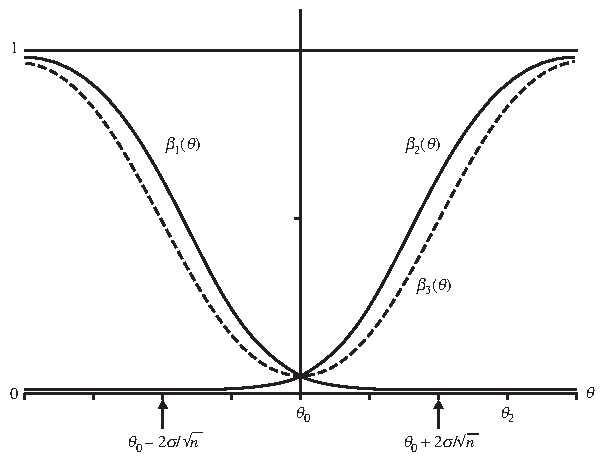
\includegraphics[width=.83\textwidth]{assets/chapter8/fig8-3-3.pdf}
\caption{\autoref{ex:8.3.19}中三个检验的功效函数. $\beta_3(\theta)$ 是一个无偏的水平 $\alpha=.05$ 检验的功效函数.}\label{fig:8.3.3}
\end{figure}

上式最后一项等于
$$P_{\theta_2}\left(\bar X<-\frac{\sigma z_\alpha}{\sqrt n}+\theta_0\right)=\beta_1(\theta_2).$$
所以检验1不是水平 $\alpha$ 的一致最强检验，因为检验2在 $\theta_2$ 处的功效更高. 前面又已证明，如果存在水平 $\alpha$ 的一致最强检验，它必为检验1. 因此本问题不存在水平 $\alpha$ 的一致最强检验.\footnote{译注：这里的不存在性结论针对非平凡水平 $0<\alpha<1$，也是上述有限正态临界点论证的适用范围. 端点 $\alpha=0$ 或 $1$ 有相应的平凡一致最强检验.}
\end{example}
\autoref{ex:8.3.19}再次说明 Neyman–Pearson 引理的用途. 先前用其充分性部分构造水平 $\alpha$ 的一致最强检验；要说明这种检验不存在，则使用其必要性部分.
\begin{example}[无偏检验]\label{ex:8.3.20}
当全部检验类中没有水平 $\alpha$ 的一致最强检验时，可以尝试在无偏检验类中寻找. 检验3当且仅当
$$\bar X>\sigma z_{\alpha/2}/\sqrt n+\theta_0\quad\text{或}\quad\bar X<-\sigma z_{\alpha/2}/\sqrt n+\theta_0$$
时，拒绝 $H_0:\theta=\theta_0$、支持 $H_1:\theta\ne\theta_0$. 其功效函数 $\beta_3(\theta)$ 与\autoref{ex:8.3.19}中的 $\beta_1(\theta),\beta_2(\theta)$ 一起画在\autoref{fig:8.3.3}中. 检验3事实上是水平 $\alpha$ 的一致最强无偏检验，即在无偏检验类中一致最强.

注意，虽然检验1和检验2在某些参数点的功效略高于检验3，但在其他参数点，检验3的功效比检验1和检验2高得多. 例如，$\beta_3(\theta_2)$ 接近一，而 $\beta_1(\theta_2)$ 接近零. 若希望在 $\theta$ 偏大或偏小时都拒绝 $H_0$，\autoref{fig:8.3.3}表明，整体而言检验3优于检验1或检验2.
\end{example}

\subsubsection{并交检验与交并检验的大小}\label{sec:8.3.3}
由于构造方式简单，并交检验（UIT）与交并检验（IUT）的大小，常可用其他一些检验的大小给出上界. 当希望得到水平 $\alpha$ 的检验、却难以求出 UIT 或 IUT 的大小时，这类界很有用.
\sourcepageanchor{351}
本节讨论这些界，并给出界可达到的例子，即检验的大小恰好等于所给界.

先考虑并交检验. 回顾，此时检验的原假设形如 $H_0:\theta\in\Theta_0$，其中 $\Theta_0=\bigcap_{\gamma\in\Gamma}\Theta_\gamma$. 具体地，设 $\lambda_\gamma(\boldsymbol x)$ 是检验 $H_{0\gamma}:\theta\in\Theta_\gamma$ 对 $H_{1\gamma}:\theta\in\Theta_\gamma^c$ 的似然比统计量，$\lambda(\boldsymbol x)$ 是检验 $H_0:\theta\in\Theta_0$ 对 $H_1:\theta\in\Theta_0^c$ 的似然比统计量. 则总体似然比检验与基于 $\lambda_\gamma(\boldsymbol x)$ 的并交检验有如下关系.
\begin{theorem}\label{thm:8.3.21}\index{SI0524@水平}
考虑检验 $H_0:\theta\in\Theta_0$ 对 $H_1:\theta\in\Theta_0^c$，其中 $\Theta_0=\bigcap_{\gamma\in\Gamma}\Theta_\gamma$，$\lambda_\gamma(\boldsymbol x)$ 如上段定义. 令 $T(\boldsymbol x)=\inf_{\gamma\in\Gamma}\lambda_\gamma(\boldsymbol x)$，构造拒绝域为
$$\{\boldsymbol x:\lambda_\gamma(\boldsymbol x)<c\text{ 对某个 }\gamma\in\Gamma\}
=\{\boldsymbol x:T(\boldsymbol x)<c\}$$
的并交检验. 再考虑拒绝域为 $\{\boldsymbol x:\lambda(\boldsymbol x)<c\}$ 的通常似然比检验. 则
\begin{enumerate}
\item\phantomsection\label{itm:thm:8.3.21:a} 对每个 $\boldsymbol x$，$T(\boldsymbol x)\ge\lambda(\boldsymbol x)$；
\item\phantomsection\label{itm:thm:8.3.21:b} 若 $\beta_T(\theta)$ 和 $\beta_\lambda(\theta)$ 分别为基于 $T$ 与 $\lambda$ 的检验的功效函数，则对每个 $\theta\in\Theta$，$\beta_T(\theta)\le\beta_\lambda(\theta)$；
\item\phantomsection\label{itm:thm:8.3.21:c} 若似然比检验的水平为 $\alpha$，则并交检验的水平也为 $\alpha$.
\end{enumerate}
\end{theorem}
\begin{proof}
由于对任意 $\gamma$，$\Theta_0=\bigcap_{\gamma\in\Gamma}\Theta_\gamma\subset\Theta_\gamma$，由\autoref{def:8.2.1}可见，对任意 $\boldsymbol x$，
$$\lambda_\gamma(\boldsymbol x)\ge\lambda(\boldsymbol x),\qquad\text{对每个 }\gamma\in\Gamma,$$
因为单独的 $\lambda_\gamma$ 的最大化范围更大. 所以 $T(\boldsymbol x)=\inf_{\gamma\in\Gamma}\lambda_\gamma(\boldsymbol x)\ge\lambda(\boldsymbol x)$，证明了\hyperref[itm:thm:8.3.21:a]{(a)}. 由\hyperref[itm:thm:8.3.21:a]{(a)}，$\{\boldsymbol x:T(\boldsymbol x)<c\}\subset\{\boldsymbol x:\lambda(\boldsymbol x)<c\}$，故
$$\beta_T(\theta)=P_\theta(T(\boldsymbol X)<c)\le P_\theta(\lambda(\boldsymbol X)<c)=\beta_\lambda(\theta),$$
证明了\hyperref[itm:thm:8.3.21:b]{(b)}. 因\hyperref[itm:thm:8.3.21:b]{(b)}对每个 $\theta$ 都成立，$\sup_{\theta\in\Theta_0}\beta_T(\theta)\le\sup_{\theta\in\Theta_0}\beta_\lambda(\theta)\le\alpha$，所以\hyperref[itm:thm:8.3.21:c]{(c)}成立.
\end{proof}
\begin{example}[一种等价性]\label{ex:8.3.22}
在某些情形下，\autoref{thm:8.3.21}中的 $T(\boldsymbol x)=\lambda(\boldsymbol x)$，由单独似然比检验构成的并交检验，与总体似然比检验相同. \autoref{ex:8.2.8}就是这种情况：由两个单侧 $t$ 检验构成的并交检验，等价于双侧似然比检验.
\end{example}
既然\autoref{thm:8.3.21}中似然比检验的功效处处不低于并交检验，可能会问为什么还要使用并交检验. 一个原因是，对每个 $\theta\in\Theta_0$，并交检验的第一类错误概率更小. 此外，若 $H_0$ 被拒绝，我们可能希望查看各个 $H_{0\gamma}$ 的单独检验，以了解原因. 至今尚未讨论关于单独 $H_{0\gamma}$ 的推断；采用这种推断程序之前，必须考察其错误概率. 但显然，逐个查看 $H_{0\gamma}$，有可能比只查看总体似然比检验获得更多信息.

现在研究交并检验的大小. 交并检验大小的一个简单界，与构造它所用的各个单独检验的大小有关. 回顾，此时原假设可写成并集，即检验
$$H_0:\theta\in\Theta_0\quad\text{对}\quad H_1:\theta\in\Theta_0^c,\qquad
\Theta_0=\bigcup_{\gamma\in\Gamma}\Theta_\gamma.$$
交并检验的拒绝域形如 $R=\bigcap_{\gamma\in\Gamma}R_\gamma$，其中 $R_\gamma$ 是检验 $H_{0\gamma}:\theta\in\Theta_\gamma$ 的拒绝域.
\begin{theorem}\label{thm:8.3.23}\index{SI0496@水平}
设拒绝域为 $R_\gamma$ 的 $H_{0\gamma}$ 检验的大小为 $\alpha_\gamma$. 则拒绝域为 $R=\bigcap_{\gamma\in\Gamma}R_\gamma$ 的交并检验，是水平 $\alpha=\sup_{\gamma\in\Gamma}\alpha_\gamma$ 的检验.
\end{theorem}
\begin{proof}
取 $\theta\in\Theta_0$，则对某个 $\gamma$ 有 $\theta\in\Theta_\gamma$，并且
$$P_\theta(\boldsymbol X\in R)\le P_\theta(\boldsymbol X\in R_\gamma)\le\alpha_\gamma\le\alpha.$$
由于 $\theta\in\Theta_0$ 任意，交并检验的水平为 $\alpha$.
\end{proof}
\sourcepageanchor{352}
通常，单独拒绝域 $R_\gamma$ 被选成对所有 $\gamma$ 都有 $\alpha_\gamma=\alpha$. 此时\autoref{thm:8.3.23}说明，所得交并检验的水平为 $\alpha$.

给出交并检验大小上界的\autoref{thm:8.3.23}，比给出并交检验大小上界的\autoref{thm:8.3.21}更有用一些. 后者只适用于由似然比检验构造的并交检验，前者则适用于任意交并检验.

\autoref{thm:8.3.21}的界是似然比检验的大小，在复杂问题中可能难以计算. 但在\autoref{thm:8.3.23}中，求上界并不必使用似然比检验：任何大小 $\alpha_\gamma$ 已知的 $H_{0\gamma}$ 检验都可使用，交并检验大小的上界便用这些已知的 $\alpha_\gamma$，$\gamma\in\Gamma$ 表示.

\autoref{thm:8.3.23}的交并检验水平为 $\alpha$，但其大小可能远小于 $\alpha$，即检验可能很保守. 下列定理给出大小恰为 $\alpha$、因而检验不过于保守的条件.
\begin{theorem}\label{thm:8.3.24}
考虑检验 $H_0:\theta\in\bigcup_{j=1}^k\Theta_j$，其中 $k$ 为有限正整数. 对每个 $j=1,\ldots,k$，设 $R_j$ 为 $H_{0j}$ 的某水平 $\alpha$ 检验的拒绝域. 假设对某个 $i=1,\ldots,k$，存在参数点列 $\theta_l\in\Theta_i$，$l=1,2,\ldots$，满足
\begin{enumerate}[label=\roman*.]
\item\phantomsection\label{itm:thm:8.3.24:i} $\lim_{l\to\infty}P_{\theta_l}(\boldsymbol X\in R_i)=\alpha$；
\item\phantomsection\label{itm:thm:8.3.24:ii} 对每个 $j=1,\ldots,k$，$j\ne i$，$\lim_{l\to\infty}P_{\theta_l}(\boldsymbol X\in R_j)=1$.
\end{enumerate}
则拒绝域为 $R=\bigcap_{j=1}^kR_j$ 的交并检验，大小为 $\alpha$.
\end{theorem}
\begin{proof}
由\autoref{thm:8.3.23}，$R$ 是水平 $\alpha$ 的检验，即
\begin{equation}\label{eq:8.3.7}\sup_{\theta\in\Theta_0}P_\theta(\boldsymbol X\in R)\le\alpha.\end{equation}
但由于所有参数点 $\theta_l$ 都满足 $\theta_l\in\Theta_i\subset\Theta_0$，
$$\begin{aligned}
\sup_{\theta\in\Theta_0}P_\theta(\boldsymbol X\in R)&\ge\lim_{l\to\infty}P_{\theta_l}(\boldsymbol X\in R)\\
&=\lim_{l\to\infty}P_{\theta_l}\left(\boldsymbol X\in\bigcap_{j=1}^kR_j\right)\\
&\ge\lim_{l\to\infty}\left[\sum_{j=1}^kP_{\theta_l}(\boldsymbol X\in R_j)-(k-1)\right]&&\text{（Bonferroni 不等式）}\\
&=(k-1)+\alpha-(k-1)&&\text{（由\hyperref[itm:thm:8.3.24:i]{(i)}与\hyperref[itm:thm:8.3.24:ii]{(ii)}）}\\
&=\alpha.
\end{aligned}$$
结合\eqref{eq:8.3.7}，可知检验的大小恰为 $\alpha$.
\end{proof}
\begin{example}[交并检验]\label{ex:8.3.25}\index{SI0495@伯努利}\index{SI0497@正态}
在\autoref{ex:8.2.9}中，令 $n=m=58$，$t=1.672$，$b=57$. 则各个单独检验的大小均约为 $\alpha=.05$. 所以，由\autoref{thm:8.3.23}，交并检验是水平 $\alpha=.05$ 的检验，即产品实际上不合格却被判为合格的概率不超过 $.05$. 事实上，这个检验的大小为 $\alpha=.05$. 为说明这一点，考虑参数点列 $\theta_l=(\theta_{1l},\theta_2)$，其中 $l\to\infty$ 时 $\theta_{1l}\to\infty$，$\theta_2=.95$. 因 $\theta_2\le.95$，所有这些点都在 $\Theta_0$ 中. 而且 $\theta_{1l}\to\infty$ 时 $P_{\theta_l}(\boldsymbol X\in R_1)\to1$；因为 $\theta_2=.95$，对所有 $l$，$P_{\theta_l}(\boldsymbol X\in R_2)=.05$. 所以由\autoref{thm:8.3.24}，交并检验的大小为 $\alpha$.\footnote{译注：本例最初已说明大小为近似值，后面的“恰为”及“不超过”不能按精确的 $.05$ 理解. 对给定 $m=58,b=57$，第二项检验在 $58$ 次均成功时拒绝，其边界概率为 $.95^{58}\approx.05105>.05$；沿原文所选参数列，交并拒绝概率也趋于这一数值，故所给检验并非严格的水平 $.05$ 检验. 原参数和结论均保留，数值近似的影响在此说明.}
\end{example}
注意，\autoref{ex:8.3.25}只利用 $X_1,\ldots,X_n$ 与 $Y_1,\ldots,Y_m$ 的边缘分布求出检验大小. 这一点非常重要，直接关系到交并检验的实用性，因为联合分布往往难以获知，即使知道也往往难以处理. 例如，若 $X_i,Y_i$ 来自同一块织物的测量，二者可能有关联；要计算某个特定参数值下交并检验的精确功效，就必须建立并使用这种关联的模型.

\sourcepageanchor{353}
\subsubsection{\texorpdfstring{$p$}{p} 值}\label{sec:8.3.4}
假设检验完成后，必须以在统计上有意义的方式报告结论. 一种报告方式是给出所用检验的大小 $\alpha$，以及拒绝或接受 $H_0$ 的决定. 检验大小包含重要信息：若 $\alpha$ 小，拒绝 $H_0$ 的决定相当有说服力；若 $\alpha$ 大，这一决定就不太有说服力，因为检验错误作出该决定的概率较大. 另一种方式是报告称为 $p$ 值（$p$-value）的某种检验统计量的取值.
\begin{definition}\label{def:8.3.26}\index{SI0742@p值}
$p$ 值 $p(\boldsymbol X)$ 是一个检验统计量，对每个样本点 $\boldsymbol x$ 满足 $0\le p(\boldsymbol x)\le1$. $p(\boldsymbol X)$ 的小值为 $H_1$ 为真提供证据. 若对每个 $\theta\in\Theta_0$ 和每个 $0\le\alpha\le1$，都有
\begin{equation}\label{eq:8.3.8}P_\theta(p(\boldsymbol X)\le\alpha)\le\alpha,\end{equation}
则称该 $p$ 值有效（valid\mbox{）.}
\end{definition}
若 $p(\boldsymbol X)$ 有效，很容易基于它构造水平 $\alpha$ 的检验. 当且仅当 $p(\boldsymbol X)\le\alpha$ 时拒绝 $H_0$ 的检验，由\eqref{eq:8.3.8}可知水平为 $\alpha$. 用 $p$ 值报告检验结果的优点是，每位读者都能选择自己认为适当的 $\alpha$，将报告的 $p(\boldsymbol x)$ 与之比较，判断这些数据会导致接受还是拒绝 $H_0$. 此外，$p$ 值越小，拒绝 $H_0$ 的证据越强. 因而，$p$ 值在一个更连续的尺度上报告检验结果，而不只是“接受 $H_0$”或“拒绝 $H_0$”这样的二分决策.

\autoref{thm:8.3.27}给出定义有效 $p$ 值最常用的方法.
\begin{theorem}\label{thm:8.3.27}
设 $W(\boldsymbol X)$ 是一个检验统计量，其大值为 $H_1$ 为真提供证据. 对每个样本点 $\boldsymbol x$，定义
\begin{equation}\label{eq:8.3.9}p(\boldsymbol x)=\sup_{\theta\in\Theta_0}P_\theta(W(\boldsymbol X)\ge W(\boldsymbol x)).\end{equation}
则 $p(\boldsymbol X)$ 是有效 $p$ 值.
\end{theorem}
\begin{proof}
固定 $\theta\in\Theta_0$. 用 $F_\theta(w)$ 表示 $-W(\boldsymbol X)$ 的累积分布函数，定义
$$\begin{aligned}
p_\theta(\boldsymbol x)&=P_\theta(W(\boldsymbol X)\ge W(\boldsymbol x))\\
&=P_\theta(-W(\boldsymbol X)\le-W(\boldsymbol x))=F_\theta(-W(\boldsymbol x)).
\end{aligned}$$
则随机变量 $p_\theta(\boldsymbol X)$ 等于 $F_\theta(-W(\boldsymbol X))$. 因此，由概率积分变换或\autoref{exercise:2.10}，$p_\theta(\boldsymbol X)$ 的分布在随机意义下大于或等于 $\operatorname{uniform}(0,1)$ 分布，即对每个 $0\le\alpha\le1$，$P_\theta(p_\theta(\boldsymbol X)\le\alpha)\le\alpha$. 因为对每个 $\boldsymbol x$，$p(\boldsymbol x)=\sup_{\theta'\in\Theta_0}p_{\theta'}(\boldsymbol x)\ge p_\theta(\boldsymbol x)$，所以
$$P_\theta(p(\boldsymbol X)\le\alpha)\le P_\theta(p_\theta(\boldsymbol X)\le\alpha)\le\alpha.$$
这对每个 $\theta\in\Theta_0$ 和每个 $0\le\alpha\le1$ 成立，故 $p(\boldsymbol X)$ 有效.
\end{proof}
\eqref{eq:8.3.9}的上确界可能难以计算. 下面两个例子说明不太困难的常见情形：第一例无需取上确界；第二例则容易确定使上确界达到的 $\theta$ 值.
\begin{example}[双侧正态检验的 $p$ 值]\label{ex:8.3.28}
设 $X_1,\ldots,X_n$ 是来自 $\mathrm n(\mu,\sigma^2)$ 总体的随机样本. 考虑检验 $H_0:\mu=\mu_0$ 对 $H_1:\mu\ne\mu_0$. 由\autoref{exercise:8.38}，似然比检验在 $W(\boldsymbol X)=|\bar X-\mu_0|/(S/\sqrt n)$ 较大时拒绝 $H_0$. 若 $\mu=\mu_0$，不论 $\sigma$ 为何，$(\bar X-\mu_0)/(S/\sqrt n)$ 均服从自由度为 $n-1$ 的 Student $t$ 分布. 因而计算\eqref{eq:8.3.9}时，对所有 $\theta$ 值，也就是所有 $\sigma$ 值，概率都相同. 所以，这个双侧 $t$ 检验由\eqref{eq:8.3.9}给出的 $p$ 值为
$$p(\boldsymbol x)=2P\left(T_{n-1}\ge\frac{|\bar x-\mu_0|}{s/\sqrt n}\right),$$
其中 $T_{n-1}$ 服从自由度为 $n-1$ 的 Student $t$ 分布.
\end{example}
\sourcepageanchor{354}
\begin{example}[单侧正态检验的 $p$ 值]\label{ex:8.3.29}
再考虑\autoref{ex:8.3.28}的正态模型，但检验 $H_0:\mu\le\mu_0$ 对 $H_1:\mu>\mu_0$. 由\autoref{exercise:8.37}，似然比检验在 $W(\boldsymbol X)=(\bar X-\mu_0)/(S/\sqrt n)$ 较大时拒绝 $H_0$. 下列论证说明，对此统计量，\eqref{eq:8.3.9}的上确界总在参数 $(\mu_0,\sigma)$ 处达到，且所取 $\sigma$ 值无关紧要. 考虑任意 $\mu\le\mu_0$ 和任意 $\sigma$：
$$\begin{aligned}
P_{\mu,\sigma}(W(\boldsymbol X)\ge W(\boldsymbol x))
&=P_{\mu,\sigma}\left(\frac{\bar X-\mu_0}{S/\sqrt n}\ge W(\boldsymbol x)\right)\\
&=P_{\mu,\sigma}\left(\frac{\bar X-\mu}{S/\sqrt n}\ge W(\boldsymbol x)+\frac{\mu_0-\mu}{S/\sqrt n}\right)\\
&=P_{\mu,\sigma}\left(T_{n-1}\ge W(\boldsymbol x)+\frac{\mu_0-\mu}{S/\sqrt n}\right)\\
&\le P(T_{n-1}\ge W(\boldsymbol x)).
\end{aligned}$$
这里 $T_{n-1}$ 仍服从自由度为 $n-1$ 的 Student $t$ 分布. 最后一行的不等式成立，是因为 $\mu_0\ge\mu$，所以 $(\mu_0-\mu)/(S/\sqrt n)$ 是非负随机变量. 此处省去 $P$ 的下标，因为该概率不依赖 $(\mu,\sigma)$. 另外，
$$\begin{aligned}
P(T_{n-1}\ge W(\boldsymbol x))&=P_{\mu_0,\sigma}\left(\frac{\bar X-\mu_0}{S/\sqrt n}\ge W(\boldsymbol x)\right)\\
&=P_{\mu_0,\sigma}(W(\boldsymbol X)\ge W(\boldsymbol x)),
\end{aligned}$$
由于 $(\mu_0,\sigma)\in\Theta_0$，这一概率正是\eqref{eq:8.3.9}取上确界时所考虑的概率之一. 因此，单侧 $t$ 检验由\eqref{eq:8.3.9}给出的 $p$ 值为
$$p(\boldsymbol x)=P(T_{n-1}\ge W(\boldsymbol x))=P\left(T_{n-1}\ge\frac{\bar x-\mu_0}{s/\sqrt n}\right).$$
\end{example}
定义有效 $p$ 值的另一种方法，是对充分统计量取条件分布，从而替代\eqref{eq:8.3.9}. 设 $S(\boldsymbol X)$ 是模型 $\{f(\boldsymbol x\mid\theta):\theta\in\Theta_0\}$ 的充分统计量. （为避免检验功效低，重要的是 $S$ 仅对原假设模型充分，而不是对整个模型 $\{f(\boldsymbol x\mid\theta):\theta\in\Theta\}$ 充分.）若原假设为真，给定 $S=s$ 后 $\boldsymbol X$ 的条件分布不依赖 $\theta$. 再令 $W(\boldsymbol X)$ 为大值支持 $H_1$ 为真的检验统计量. 对每个样本点 $\boldsymbol x$ 定义
\begin{equation}\label{eq:8.3.10}\index{SI0743@条件}p(\boldsymbol x)=P(W(\boldsymbol X)\ge W(\boldsymbol x)\mid S=S(\boldsymbol x)).\end{equation}
像\autoref{thm:8.3.27}那样论证，但只考虑给定 $S=s$ 后 $\boldsymbol X$ 的这一个条件分布，可知对任意 $0\le\alpha\le1$，
$$P(p(\boldsymbol X)\le\alpha\mid S=s)\le\alpha.$$
于是，对任意 $\theta\in\Theta_0$，无条件地有
$$\begin{aligned}
P_\theta(p(\boldsymbol X)\le\alpha)&=\sum_sP(p(\boldsymbol X)\le\alpha\mid S=s)P_\theta(S=s)\\
&\le\sum_s\alpha P_\theta(S=s)\le\alpha.
\end{aligned}$$
所以，\eqref{eq:8.3.10}定义的 $p(\boldsymbol X)$ 有效. 对连续 $S$，求和可换成积分，但此法通常用于离散 $S$，如下例.
\begin{example}[Fisher 精确检验]\label{ex:8.3.30}
设 $S_1,S_2$ 是独立观测，$S_1\sim\operatorname{binomial}(n_1,p_1)$，$S_2\sim\operatorname{binomial}(n_2,p_2)$. 考虑检验 $H_0:p_1=p_2$ 对 $H_1:p_1>p_2$. 在 $H_0$ 下，用 $p$ 表示 $p_1=p_2$ 的共同值，$(S_1,S_2)$ 的联合质量函数为
$$\begin{aligned}
f(s_1,s_2\mid p)&=\binom{n_1}{s_1}p^{s_1}(1-p)^{n_1-s_1}\binom{n_2}{s_2}p^{s_2}(1-p)^{n_2-s_2}\\
&=\binom{n_1}{s_1}\binom{n_2}{s_2}p^{s_1+s_2}(1-p)^{n_1+n_2-(s_1+s_2)}.
\end{aligned}$$
\sourcepageanchor{355}
因此，$S=S_1+S_2$ 在 $H_0$ 下是充分统计量. 给定 $S=s$，合理的做法是用 $S_1$ 作检验统计量，当 $S_1$ 较大时拒绝 $H_0$、支持 $H_1$，因为较大的 $S_1$ 对应较小的 $S_2=s-S_1$. 给定 $S=s$ 后 $S_1$ 的条件分布为 $\operatorname{hypergeometric}(n_1+n_2,n_1,s)$（见\autoref{exercise:8.48}\mbox{）.} 所以，\eqref{eq:8.3.10}中的条件 $p$ 值为
$$p(s_1,s_2)=\sum_{j=s_1}^{\min\{n_1,s\}}f(j\mid s),$$
即超几何概率之和. 由这个 $p$ 值定义的检验称为 Fisher 精确检验（Fisher's Exact Test\mbox{）.}
\end{example}

\subsubsection{损失函数意义下的最优性}\label{sec:8.3.5}\index{SI0244@决策论}\index{SI0492@决策论}
可以像\autoref{sec:7.3.4}那样，通过决策论分析来比较假设检验，而不只通过功效函数比较. 为作这种分析，必须为假设检验问题指定行动空间和损失函数.

假设检验问题只允许两种行动：“接受 $H_0$”或“拒绝 $H_0$”，可分别记为 $a_0,a_1$. 行动空间是两点集合 $\mathscr A=\{a_0,a_1\}$.\index{SI0004@行动空间}\semanticindexanchor{4:355} 决策规则 $\delta(\boldsymbol x)$（一个假设检验）是样本空间 $\mathscr X$ 上只取 $a_0,a_1$ 两个值的函数. 集合 $\{\boldsymbol x:\delta(\boldsymbol x)=a_0\}$ 是接受域，$\{\boldsymbol x:\delta(\boldsymbol x)=a_1\}$ 是拒绝域，正如\autoref{def:8.1.3}.

假设检验问题的损失函数应反映：若 $\theta\in\Theta_0$ 却选择 $a_1$，或 $\theta\in\Theta_0^c$ 却选择 $a_0$，就犯了错误；另外两种可能情形则作出了正确决定. 由于只有两种可能行动，损失函数 $L(\theta,a)$ 只含两部分. $L(\theta,a_0)$ 是决定接受 $H_0$ 时，在不同 $\theta$ 值下产生的损失；$L(\theta,a_1)$ 则是决定拒绝 $H_0$ 时的损失.

检验问题中最简单的损失称为 $0$–$1$ 损失（$0$–$1$ loss），定义为
$$L(\theta,a_0)=\begin{cases}0,&\theta\in\Theta_0,\\1,&\theta\in\Theta_0^c,\end{cases}
\qquad L(\theta,a_1)=\begin{cases}1,&\theta\in\Theta_0,\\0,&\theta\in\Theta_0^c.\end{cases}$$
采用 $0$–$1$ 损失时，正确决定的损失为 $0$，错误决定的损失为 $1$. 这是两类错误后果相同的一种特别简单的情形. 稍微更现实的损失，是为两类错误赋予不同代价的广义 $0$–$1$ 损失（generalized $0$–$1$ loss）：
\begin{equation}\label{eq:8.3.11}\index{SI0655@广义零一}\index{SI0656@假设检验}\index{SI0663@零一}
L(\theta,a_0)=\begin{cases}0,&\theta\in\Theta_0,\\c_{\mathrm{II}},&\theta\in\Theta_0^c,\end{cases}
\qquad L(\theta,a_1)=\begin{cases}c_{\mathrm I},&\theta\in\Theta_0,\\0,&\theta\in\Theta_0^c.\end{cases}
\end{equation}
这里 $c_{\mathrm I}$ 是第一类错误、即错误拒绝 $H_0$ 的代价，$c_{\mathrm{II}}$ 是第二类错误、即错误接受 $H_0$ 的代价. （实际上，比较检验时真正重要的只是比值 $c_{\mathrm{II}}/c_{\mathrm I}$，不是两个单独的值. 若 $c_{\mathrm I}=c_{\mathrm{II}}$，实质上就是 $0$–$1$ 损失.）

决策论分析用风险函数（期望损失）评价假设检验程序. 检验的风险函数与功效函数密切相关，如下列分析所示.

设 $\beta(\theta)$ 是基于决策规则 $\delta$ 的检验的功效函数，即若用 $R=\{\boldsymbol x:\delta(\boldsymbol x)=a_1\}$ 表示拒绝域，则
$$\beta(\theta)=P_\theta(\boldsymbol X\in R)=P_\theta(\delta(\boldsymbol X)=a_1).$$
\sourcepageanchor{356}

\begin{figure}[htbp]\centering
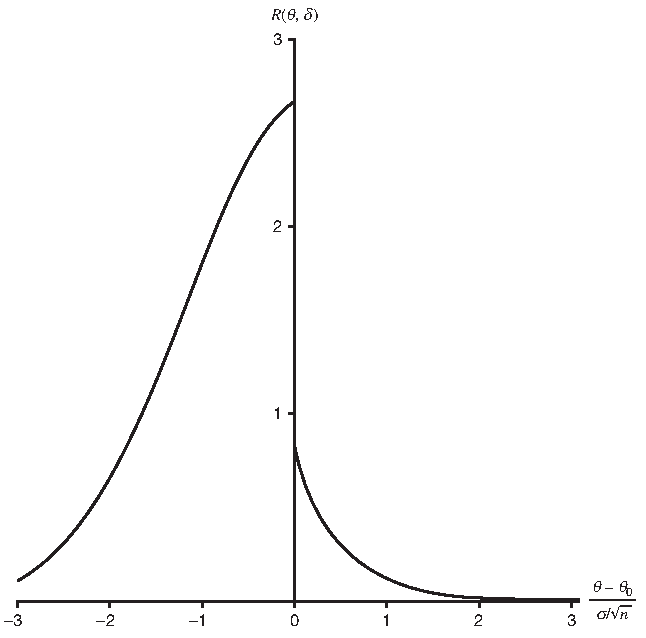
\includegraphics[width=.8\textwidth]{assets/chapter8/fig8-3-4.pdf}
\caption{\autoref{ex:8.3.31}中检验的风险函数，其中 $z=\sqrt n(\theta-\theta_0)/\sigma$.}\label{fig:8.3.4}
\end{figure}

与\eqref{eq:8.3.11}相应、特别是与 $0$–$1$ 损失相应的风险函数非常简单. 对任意 $\theta\in\Theta$，$L(\theta,a)$ 只取两个值：若 $\theta\in\Theta_0$，为 $0$ 和 $c_{\mathrm I}$；若 $\theta\in\Theta_0^c$，为 $0$ 和 $c_{\mathrm{II}}$. 所以风险为
\begin{equation}\label{eq:8.3.12}\index{SI0505@与风险的关系}
\begin{aligned}
R(\theta,\delta)&=0P_\theta(\delta(\boldsymbol X)=a_0)+c_{\mathrm I}P_\theta(\delta(\boldsymbol X)=a_1)\\
&=c_{\mathrm I}\beta(\theta),&&\theta\in\Theta_0;\\
R(\theta,\delta)&=c_{\mathrm{II}}P_\theta(\delta(\boldsymbol X)=a_0)+0P_\theta(\delta(\boldsymbol X)=a_1)\\
&=c_{\mathrm{II}}(1-\beta(\theta)),&&\theta\in\Theta_0^c.
\end{aligned}
\end{equation}
决策论方法与更传统的功效方法之间的这种相似性，部分归因于损失函数的形式. 但如下所示，在所有假设检验问题中，功效函数都在风险函数中起重要作用.
\begin{example}[一致最强检验的风险]\label{ex:8.3.31}\index{SI0493@均值}
设 $X_1,\ldots,X_n$ 是来自 $\mathrm n(\mu,\sigma^2)$ 总体的随机样本，$\sigma^2$ 已知.\footnote{译注：本例原文开头用 $\mu$ 表示正态均值，随后检验与功效公式改用 $\theta$；应理解为同一均值参数，原记号保留.} 检验 $H_0:\theta\ge\theta_0$ 对 $H_1:\theta<\theta_0$ 的水平 $\alpha$ 一致最强检验，在 $(\bar X-\theta_0)/(\sigma/\sqrt n)<-z_\alpha$ 时拒绝 $H_0$（\autoref{ex:8.3.15}\mbox{）.} 其功效函数为
$$\beta(\theta)=P_\theta\left(Z<-z_\alpha-\frac{\theta-\theta_0}{\sigma/\sqrt n}\right),$$
其中 $Z\sim\mathrm n(0,1)$. 对 $\alpha=.10$，取 $c_{\mathrm I}=8$、$c_{\mathrm{II}}=3$ 时，\eqref{eq:8.3.12}的风险函数见\autoref{fig:8.3.4}. 注意风险函数在 $\theta=\theta_0$ 处不连续；这是因为在 $\theta_0$ 处表达式由 $\beta(\theta)$ 变为 $1-\beta(\theta)$，并且 $c_{\mathrm I}$ 与 $c_{\mathrm{II}}$ 不同.
\end{example}
\sourcepageanchor{357}
$0$–$1$ 损失只判断决定是对还是错. 某些错误决定可能比其他错误决定更严重，损失函数应反映这一点. 检验 $H_0:\theta\ge\theta_0$ 对 $H_1:\theta<\theta_0$ 时，若 $\theta$ 略大于 $\theta_0$ 而拒绝 $H_0$，虽犯第一类错误，却可能不很严重；若 $\theta$ 远大于 $\theta_0$，拒绝 $H_0$ 的不良后果可能严重得多. 反映这种情况的一个损失函数是
\begin{equation}\label{eq:8.3.13}
L(\theta,a_0)=\begin{cases}0,&\theta\ge\theta_0,\\b(\theta_0-\theta),&\theta<\theta_0,\end{cases}
\quad L(\theta,a_1)=\begin{cases}c(\theta-\theta_0)^2,&\theta\ge\theta_0,\\0,&\theta<\theta_0,\end{cases}
\end{equation}
其中 $b,c$ 为正常数. 例如，若实验者检验某药物是否降低胆固醇水平，可以这样设定 $H_0,H_1$，取 $\theta_0$ 为可接受胆固醇水平的标准. 因高胆固醇水平与心脏病相关，在 $\theta$ 很大时拒绝 $H_0$ 的后果相当严重. \eqref{eq:8.3.13}这样的损失函数反映了这一后果. \hyperref[bib:source320]{Vardeman (1987)} 主张使用类似类型的损失函数.

即使对\eqref{eq:8.3.13}这样的一般损失函数，风险函数与功效函数仍密切相关. 对任意固定 $\theta$，损失不是 $L(\theta,a_0)$，就是 $L(\theta,a_1)$，所以期望损失为
\begin{equation}\label{eq:8.3.14}
\begin{aligned}
R(\theta,\delta)&=L(\theta,a_0)P_\theta(\delta(\boldsymbol X)=a_0)+L(\theta,a_1)P_\theta(\delta(\boldsymbol X)=a_1)\\
&=L(\theta,a_0)(1-\beta(\theta))+L(\theta,a_1)\beta(\theta).
\end{aligned}
\end{equation}
评价假设检验时，功效函数总是重要的；但在决策论分析中，损失函数赋予的权重也同样重要.

